%
%
%

\begin{frame}[t,allowframebreaks]{Biological inspirations - }

    % \begin{itemize}
    % \item
    In mammalian brain, 
    sensory input from the eyes 
    is received by the 
    \index{lateral geniculate nucleus}\gls{lateral geniculate nucleus}
    connecting the thalamus with the optic nerve.\\
    \vspace{0.2cm}
    % \item
    Subsequently, sensory input is passed to the \index{visual cortex}\gls{visual cortex},
    the area of the \index{cerebral cortex}\gls{cerebral cortex} that 
    processes visual information.\\
    % \end{itemize}

    \begin{columns}
        \begin{column}{0.38\textwidth}
         \begin{center}
          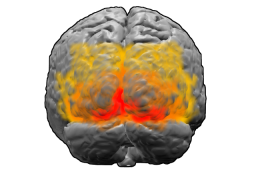
\includegraphics[width=1.0\textwidth]
          {./images/biological_inspirations/brodmann_areas_17_18_19.png}\\
          {\scriptsize 
          Rear view of the brain:\\
          Brodmann area 17 (red); area 18 (orange); area 19 (yellow).\\
          \color{col:attribution} 
          Image reproduced from \cite{Wikipedia:VisualCortex}}\\
         \end{center}
        \end{column}
        \begin{column}{0.62\textwidth}
            \vspace{0.2cm}
            \small
            The visual cortex includes several areas:
            \begin{itemize}
                \small
                \item The area that receives the sensory input is  
                 the \index{primary visual cortex}\gls{primary visual cortex}. 
                 It is also known as the
                 \index{visual area 1 (V1)} \gls{visual area 1 (V1)}, 
                 \index{Brodmann area 17} \gls{Brodmann area 17}, or 
                 \index{striate cortex} \gls{striate cortex}.
                \item
                 From V1, information is transmitted along 2 main pathways
                 to the the extrastriate cortex which consist of:
                 \begin{itemize}
                    \item Brodmann area 18, or visual area 2 (V2)
                    \item Brodmann area 19, or visual areas 3, 4 and 5 (V3-V5)
                \end{itemize}                    
            \end{itemize}                
        \end{column}
    \end{columns}


    \framebreak

    \index{CNN}\index{convolutional neural network}\glspl{cnn} 
    were inspired by studies of the 
    \index{primary visual cortex}\gls{primary visual cortex}
    of animals
    by \index{Hubel}\gls{Hubel} 
    and \index{Wiesel}\gls{Wiesel}\cite{Hubel:1959v1,Hubel:1962v1}.

    In a series of experiments, they studied the visual cortex by 
    \begin{itemize}
    \item {\bf projecting visual stimuli} on the 
      eyes of anaesthetized cats, and
    \item {\bf measuring the activity of neurons} by recording signals 
      on electrodes inserted in the brain.
    \end{itemize}

    \begin{columns}
        \begin{column}{0.55\textwidth}
            \begin{center}
            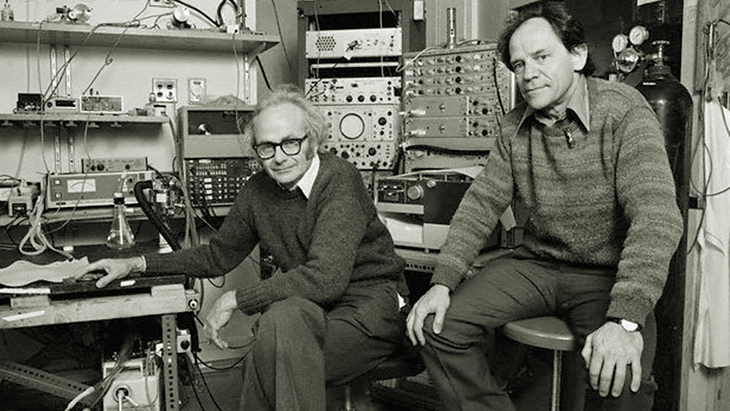
\includegraphics[width=0.9\textwidth]
                {./images/people/hubel_and_weisel.png}\\
            {\scriptsize 
            Hubel and Weisel.\\
            \color{col:attribution} 
            Photo from \cite{HarvardBrainTour:HubelAndWiesel}}\\
            \end{center}
        \end{column}
        \begin{column}{0.40\textwidth}
            \begin{center}
            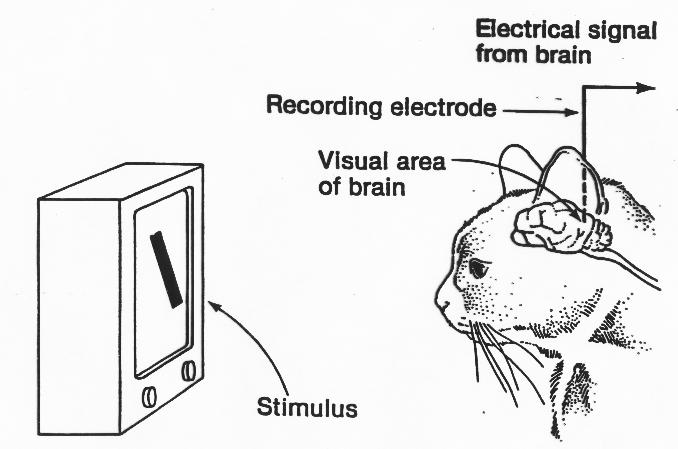
\includegraphics[width=1.0\textwidth]
                {./images/biological_inspirations/hubel_wiesel_experiment.png}\\
            {\scriptsize 
            Hubel and Wiesel experiment.\\
            \color{col:attribution} 
            Schematic from \cite{GoodPsychology:HubelAndWiesel}}\\
            \end{center}
        \end{column}
    \end{columns}

    \framebreak

    \index{Hubel}\gls{Hubel} and \index{Wiesel}\gls{Wiesel} 
    established the existence of {\bf orientation selectivity} 
    and {\bf columnar organization} of the 
    \index{primary visual cortex}\gls{primary visual cortex}.\\

    Key observations:
    \begin{itemize}
        \item Cells are arranged in columns.
        \item Colums are grouped together in hypercolumns, 
          each occupying a 2 mm x 2 mm area of the cerebral cortex.
        \item Each small area of the visual field is mapped to a hypercolumn.
        \item There are different types of cells:
        \begin{itemize}
            \item {\em Simple} cells responding best to elongated
               bars or edges of light or dark 
               that have a preferred orientation and location.
            \item {\em Complex} cells 
               receiving inputs from a collection of simple cells 
               with the same preferred orientation but 
               different preferred locations
        \end{itemize} 
    \end{itemize} 

    \begin{blockexample}{}
        \small
        \gls{Hubel} and \gls{Wiesel} were awarded the 1981 Nobel prize for Physiology.\\
        Details in \url{https://www.nobelprize.org/prizes/medicine/1981/}.
    \end{blockexample}

    \framebreak

    V1 performs a simple filtering to {\bf enhance edges and contours}.

\end{frame}
